\documentclass[11pt]{article}
 
\newcommand\CG[1]{\textcolor{red}{#1}}

\usepackage{lineno,hyperref}

\usepackage[margin=1 in]{geometry}
\renewcommand{\baselinestretch}{1.25}

\usepackage{authblk}
\usepackage{galois} % composition function \comp
\usepackage{bm}
\usepackage{amsmath}
\usepackage{amssymb}
\usepackage{mathrsfs}
\usepackage{amsthm}
\usepackage{natbib}
\usepackage{graphicx}
\usepackage{color}
\usepackage{booktabs}
\usepackage[page,title]{appendix}
%\renewcommand\appendixname{haha}
\usepackage{enumerate}
\usepackage{changepage}
\usepackage{datetime}
\newdate{date}{7}{15}{2020}

\usepackage{listings}

%%%%%%%%%%%%%%  Notations %%%%%%%%%%
\DeclareMathOperator{\mytr}{tr}
\DeclareMathOperator{\mydiag}{diag}
\DeclareMathOperator{\myrank}{Rank}
\DeclareMathOperator{\myP}{P}
\DeclareMathOperator{\myE}{E}
\DeclareMathOperator{\myVar}{Var}
\DeclareMathOperator*{\argmax}{arg\,max}
\DeclareMathOperator*{\argmin}{arg\,min}


\newcommand{\Ba}{\mathbf{a}}    \newcommand{\Bb}{\mathbf{b}}    \newcommand{\Bc}{\mathbf{c}}    \newcommand{\Bd}{\mathbf{d}}    \newcommand{\Be}{\mathbf{e}}    \newcommand{\Bf}{\mathbf{f}}    \newcommand{\Bg}{\mathbf{g}}    \newcommand{\Bh}{\mathbf{h}}    \newcommand{\Bi}{\mathbf{i}}    \newcommand{\Bj}{\mathbf{j}}    \newcommand{\Bk}{\mathbf{k}}    \newcommand{\Bl}{\mathbf{l}}
\newcommand{\Bm}{\mathbf{m}}    \newcommand{\Bn}{\mathbf{n}}    \newcommand{\Bo}{\mathbf{o}}    \newcommand{\Bp}{\mathbf{p}}    \newcommand{\Bq}{\mathbf{q}}    \newcommand{\Br}{\mathbf{r}}    \newcommand{\Bs}{\mathbf{s}}    \newcommand{\Bt}{\mathbf{t}}    \newcommand{\Bu}{\mathbf{u}}    \newcommand{\Bv}{\mathbf{v}}    \newcommand{\Bw}{\mathbf{w}}    \newcommand{\Bx}{\mathbf{x}}
\newcommand{\By}{\mathbf{y}}    \newcommand{\Bz}{\mathbf{z}}    
\newcommand{\bA}{\mathbf{A}}    \newcommand{\bB}{\mathbf{B}}    \newcommand{\bC}{\mathbf{C}}    \newcommand{\bD}{\mathbf{D}}    \newcommand{\bE}{\mathbf{E}}    \newcommand{\bF}{\mathbf{F}}    \newcommand{\bG}{\mathbf{G}}    \newcommand{\bH}{\mathbf{H}}    \newcommand{\bI}{\mathbf{I}}    \newcommand{\bJ}{\mathbf{J}}    \newcommand{\bK}{\mathbf{K}}    \newcommand{\bL}{\mathbf{L}}
\newcommand{\bM}{\mathbf{M}}    \newcommand{\bN}{\mathbf{N}}    \newcommand{\bO}{\mathbf{O}}    \newcommand{\bP}{\mathbf{P}}    \newcommand{\bQ}{\mathbf{Q}}    \newcommand{\bR}{\mathbf{R}}    \newcommand{\bS}{\mathbf{S}}    \newcommand{\bT}{\mathbf{T}}    \newcommand{\bU}{\mathbf{U}}    \newcommand{\bV}{\mathbf{V}}    \newcommand{\bW}{\mathbf{W}}    \newcommand{\bX}{\mathbf{X}}
\newcommand{\bY}{\mathbf{Y}}    \newcommand{\bZ}{\mathbf{Z}}    

\newcommand{\bfsym}[1]{\ensuremath{\boldsymbol{#1}}}

 \def\balpha{\bfsym \alpha}
 \def\bbeta{\bfsym \beta}
 \def\bgamma{\bfsym \gamma}             \def\bGamma{\bfsym \Gamma}
 \def\bdelta{\bfsym {\delta}}           \def\bDelta {\bfsym {\Delta}}
 \def\bfeta{\bfsym {\eta}}              \def\bfEta {\bfsym {\Eta}}
 \def\bmu{\bfsym {\mu}}                 \def\bMu {\bfsym {\Mu}}
 \def\bnu{\bfsym {\nu}}
 \def\btheta{\bfsym {\theta}}           \def\bTheta {\bfsym {\Theta}}
 \def\beps{\bfsym \varepsilon}          \def\bepsilon{\bfsym \varepsilon}
 \def\bsigma{\bfsym \sigma}             \def\bSigma{\bfsym \Sigma}
 \def\blambda {\bfsym {\lambda}}        \def\bLambda {\bfsym {\Lambda}}
 \def\bomega {\bfsym {\omega}}          \def\bOmega {\bfsym {\Omega}}
 \def\brho   {\bfsym {\rho}}
 \def\btau{\bfsym {\tau}}
 \def\bxi{\bfsym {\xi}}
 \def\bzeta{\bfsym {\zeta}}
% May add more in future.
%%%%%%%%%%%%%%%%%%%%%%%%%%%%%%%%%%%%



\theoremstyle{plain}
\newtheorem{theorem}{\quad\quad Theorem}
\newtheorem{proposition}{\quad\quad Proposition}
\newtheorem{corollary}{\quad\quad Corollary}
\newtheorem*{lemma}{\quad\quad Lemma}
\newtheorem{example}{Example}
\newtheorem{assumption}{\quad\quad Assumption}
\newtheorem{condition}{\quad\quad Condition}

\theoremstyle{definition}
\newtheorem{remark}{\quad\quad Remark}
\theoremstyle{remark}



\title{Response to Reviewers\\
    ``
    On the Wilks phenomenon of Bayes factors and the integrated likelihood ratio test
    ''
}



\author[1,2]{Rui Wang}
\author[2,3]{Xingzhong Xu}
\affil[1]{
    School of Statistics, Renmin University of China, Beijing
    100872, China
}

\affil[2]{
School of Mathematics and Statistics, Beijing Institute of Technology, Beijing 
    100081,China
}

\affil[3]{
Beijing Key Laboratory on MCAACI, Beijing Institute of Technology, Beijing 100081,China
}



\begin{document}
\maketitle
We are grateful to the AE for informing us a number of useful relevant papers and helpful comments.
He/she even provided us an example, namely binomial mixture model, which is very suitable for illustrating the advantages of the proposed method over the LRT.
We thank both reviewers for their valuable and helpful comments and critiques.
We have carefully revised our paper according to the comments and critiques and have made extensive modifications on the original manuscript.
Now the paper is much improved.
Below we respond to the AE and each reviewer in turn.

\section{Response to the AE}
\textbf{
    First, the fractional posterior is a special case of a Gibbs posterior, and $\sqrt{n}$ consistency of Gibbs posteriors has been around in the literature for a while; see, for example, the paper "An MCMC approach to classical estimation" by Chernozhukov and Hong as a representative example. This is particularly not surprising for the fractional posterior since roughly speaking, it keeps the center of the posterior unaffected for large n and reduces the variance by a scale
    factor depending on the fractional power - hence the classical Bernstein--von Mises phenomenon should go through for the fractional posterior under the same conditions as the exact posterior. I found the integrability condition in Proposition 2 to be somewhat strong in this regard.
}

\textbf{Answers:}
We thank the AE for informing the literature on the Gibbs posterior.
The fact that the fractional posterior is a special case of a Gibbs posterior is interesting, and we mention this connection in the revised paper.
I found that the results of \cite{Chernozhukov2003} require certain conditions on the likelihood and only bounded likelihood can satisfy their conditions.
Since we would like to include the unbounded likelihood case, we can not use the $\sqrt{n}$ consistency result in their paper.
We note that the assumptions of \cite{Chernozhukov2003} (that is, compact parameter space and continuous prior density) implies that the prior distribution is proper.
In fact, we found that most existing results on the consistency of posterior require that the prior is proper.
Since improper priors are often used for Bayes factor, existing results are not suitable for our purpose.
The integrability condition in Proposition 2 is
\begin{align*}
    \int_{\Theta} \exp\{ - c^* D_{1-t}(\theta_0 \| \theta )\} \pi(\theta) \, \mathrm d \theta < \infty.
\end{align*}
Note that if $\pi(\theta)$ is proper, then
\begin{align*}
    \int_{\Theta} \exp\{ - c^* D_{1-t}(\theta_0 \| \theta )\} \pi(\theta) \, \mathrm d \theta <
    \int_{\Theta} \pi(\theta) \, \mathrm d \theta = 1 < \infty.
\end{align*}
Hence the integrability condition is satisfied for any proper priors.
Furthermore, it also allows improper priors provided the tail of the prior density is not too thick.
Hence our integrability condition is very weak.
In the revised paper, we add a remark on this condition.


\textbf{
    The paper doesn't discuss recent advances in the frequentist literature. I would point out the article "Generalized likelihood ratio statistics and Wilks phenomenon" by Fan et al. as an example; this has been cited many times and the authors need to check what is there beyond the usual LRT. Also take a look at the paper "Geometric Understanding of Likelihood Ratio Statistics" by Fan et al. which among other things provides a Bayesian argument for the derivation of the classical Wilk's phenomenon.
}

\textbf{Answers:}
We thank the AE for informing us these references.
%, which are reviewed in the revised paper.
In the revised paper, we have improved the literature review on the LRT.
Although the LRT is a very classical idea, we found that the LRT is an active research topic very recently, with important advances both in theory \cite{Sur2019The,Anastasiou2020Bounds} and methodology \cite{Wasserman2020}.
Compared with the LRT, the test method of \cite{Wasserman2020} is very general, and can be used in complex models, such as mixture models.
As \cite{Wasserman2020} noted, the generality of their method comes at the price of relatively low power.
Theses points are discussed in the revised paper.

\section{Response to reviewer 1}

\textbf{Major comments:}

\textbf{1.
    (Literature review) The paper proposes to use the Bayes factor as a test statistic for a significance test of the composite null hypothesis. I can hardly believe this idea is new. The paper does not mention any papers on this idea. I suggest to review the literature of significance test using Bayes factors or related issues. I also suggest to review the literature of large sample properties of Bayes factor, and to compare the results of this paper with existing results in the literature.
}

\textbf{Answers:}
Following the reviewer's suggestions, we improved the literature review in the revised paper.
The idea of using the Bayes factor as a test statistic is definitely not a new one, and we point out this point explicitly in the revised paper.
We add the following comment in the revised paper:
\begin{adjustwidth}{1.5em}{1.5em}
    \emph{
The idea is not new.                                                                                      
In fact, this methodology dates back at least to \cite{Good1967}, and has been considered by many
researchers since then.
\cite{Good1992} gave a review for some early literature using this idea.                                  
See \cite{Aerts2004}, \cite{zhou2018On} and \cite{Wang2020} for some recent applications of the idea. 
However, the idea has been mostly used for specific models and has not been systematically and rigorously studied for general models.                                  
One reason for this fact may be the Lindley's paradox, that is, the distribution of the Bayes factor depends heavily on the prior density; see, e.g., \cite{Shafer1982}. \ldots
}
\end{adjustwidth}

Following the reviewer's suggestion, we also comment on the literature of large sample properties of Bayes factor, as follow:
\begin{adjustwidth}{1.5em}{1.5em}
    \emph{
        In this work, we treat the Bayes factor and its variants as frequentist test statistics.
        Hence a closely related area of research is the frequentist properties of the Bayes factor.
        Most existing results in this area focus on the consistency of the Bayes factor, that is, as the sample size $n$  goes to infinity, the Bayes factor converges to $0$ under the null hypothesis, and converges to $+\infty$ under the alternative hypothesis; see \cite{berger2003approximations}, \cite{moreno2010},      \cite{WangMin2016}, \cite{Chatterjee2017} and the references therein.
        There are still relatively few researches on the asymptotic distribution of the Bayes factor.
        \cite{clarke1990information} derived the asymptotic distribution of the ratio of the marginal likelihood to the likelihood at the true parameter, which can be regarded as the Bayes factor for a point null hypothesis.
        \cite{Gelfand1994} derived formal approximations to the Bayas factor and some of its variants.
        In this work, in order to use the Bayes factor to construct frequentist tests, we give a thorough study of the asymptotic distribution of the Bayes factor and its variants for general models.
        Thess results are interesting in their own right.
}
\end{adjustwidth}

We add a remark below Theorem $1$ which gives a comparison of Theorem $1$ and the result in \cite{clarke1990information}:
\begin{adjustwidth}{1.5em}{1.5em}
    \emph{
            \cite{clarke1990information} 
            derived the asymptotic null distribution of 
            $$
            \frac{
                    {\int_{\Theta} p_n(\bX^{n}\theta) \pi(\theta)\, \mathrm d\theta}
            }
            {p_n(\bX^{n}\theta_0)}
            ,
            $$
            which can be regarded as the Bayes factor for the point null hypothesis, i.e., $p_0 = 0$.
            Theorem 1 extends their result and gives the asymptotic distribution of the general Bayes factor under both the null       hypothesis and the local alternative hypothesis.
            \cite{clarke1990information} imposed some conditions on the likelihood around the true parameter, which may not be easy to verify for some    moderately complex models.
            In comparison, Theorem 1 only assumes the likelihood can be expanded in a $n^{-1/2}$ neighborhood of the true parameter,   which is satisfied by most regular models.
}
\end{adjustwidth}

\textbf{
    2.
    (numerical examples: simulation studies and real applications) The paper does not have any numerical study. I suggest to include extensive simulation studies comparing existing significance tests such as the likelihood ratio test (LRT). If the Bayes factors in the paper are used in hypothesis testing, is there anything that the user needs to be careful about? Please include in simulation study examples in which LRT fails and examples with wide applications.
}

\textbf{Answers:}
We follow the reviewer's suggestion.
In the revised paper, we add simulations to examine the performance of the proposed method and compare it with the LRT.
The simulation examples include the logistic regression model which is an example with wide applications, and the normal mixture model and the binomial mixture model which are examples that the LRT has irregular behavior.
%For these models, researchers have proved that the LRT has irregular behavior.
%The testing problem for binomial mixture model has applications in genetics.
Numerical results show that the proposed method has good performance in terms of both test level and test power.

In the revised paper, we also discussed that the users needs to be careful about the degree of freedom when they deal with irregular models, as follows:

\begin{adjustwidth}{1.5em}{1.5em}
    \emph{
The proposed method is quite universal. 
However, when applied to irregular models, one needs to be careful about the freedom of the asymptotic chi-squared distribution.
For example, in Proposition 5 and Proposition 6, the freedom of the asymptotic chi-squared distribution is $1$ instead of $p-p_0 = 2$.
This phenomenon is essentially caused by the loss of identifiability of the mixture models.
In general, when the model has a loss of identifiability, the degree of freedom of the asymptotic chi-squred distribution may be less than $p-p_0$.
In this case, if the true degree of freedom is not easy to obtain, the user can simply use $p-p_0$ as the degree of freedom, and the resulting test can still preserve the test level.
Of course, this simple strategy may lead to decreased power.
}
\end{adjustwidth}


\textbf{
    3. (Choice of $a$ and $b$) According to Theorem $2$, there are many $a$ and $b$ such that $\Delta_{a,b}$ satisfies the Wilks phenomenon.
    In actual testing problem, what values of $a$ and $b$ would you suggest to use?
}

\textbf{Answers:}

Our results imply that the choice of $a$ and $b$ does not affect the Wilks phenomenon and asymptotic power provided $a$ and $b$ are fixed and $0<b<a<1$.
In the simulation studies of the revised paper, the default value is $a=2/3$ and $b= 1/3$.
we also add a simulation to examine the effect of $a$ and $b$ on the finite sample performance of the test procedure.
It turns out that the proposed methdod is not sensitive to the choice $a$ and $b$.
In practice, if there is no practical evidence for the choice of $a$ and $b$, one can simply choose $a = 2/3$ and $b = 1/3$.

\textbf{
    4. The paper discusses the fractional Bayes factor, the posterior Bayes factor and the integrated Bayes factor, but does not discuss the intrinsic Bayes factor. I suggest to include some discussion on the intrinsic Bayes factor. Can you get similar asymptotic results for the intrinsic Bayes factor?
}

\textbf{Answers:}
%The asymptotic behavior of the intrinsic Bayes factor is relatively simple.
%In the asymptotic sense, the intrinsic Bayes factor is equivalent to the Bayes factor with intrinsic priors; see, e.g., \cite{intrisicBayesFactor} and \cite{Moreno1998An}.
%Simple examples show that the Bayes factor with intrinsic  priors does not have Wilks phenomenon.
We follow the reviewer's suggestion.
In Appendix D of the revised paper, we rigorously derive the asymptotic distribution of the intrinsic Bayes factor.
This theoretical result is obtained by applying the law of large numbers of $U$-statistics. 
Unfortunately, it turns out that the intrinsic Bayes factor does not have Wilks phenomenon in general.
Hence intrinsic Bayes factor can not be directly used as a frequentist test statistic.
This point is made clear in our revised paper.

\textbf{
    5. The paper gives one example (mixtures of normals) for which the LRT fails. One example for the argument for the Bayes factor as the test statistic is weak. Please give more examples and numerical examples.
}

\textbf{Answers:}
We follow the reviewer's suggestion.
In the revised paper, we add two examples, the logistic regression model and the binomial mixture model.
The logistic regression model is widely used in applications.
%Although this is a sufficiently regular model, the .
%the LRT still has undesired properties.
We note that when using R language to fit a logistic regression, the $p$-value reported by the method ``\texttt{summary.glm}'' is based on the Wald test.
It is known that for logistic regression, the MLE does not exist when the data points are completely separated or quasi-completely separated; see, e.g., \cite{Albert1984On,Candes2020The_phase}.
As a consequence of this phenomenon, the Wald test has undesirable behavior.
In contrast, the generalized FBF does not rely on the estimation of the parameter, it turns out that it works well for this model.
%We proved that the proposed method has Wilks phenomenon in this problem.
%We also conduct simulations to examine the performance of the proposed method.
The binomial mixture model is useful in genetics.
It is known that the LRT for this model has complicated behavior.
For these two models, we proved that the proposed method has Wilks phenomenon.
We also conduct simulations to examine the good performance of the proposed method.
%It turns out that the proposed method has good performance in terms of both test level and test power.

\textbf{Minor comments:}

\textbf{
1. 
P. 3. L. 19. variantional $\rightarrow$ variational
}

\textbf{Answers:}
The correction has been made.

\textbf{
2. Assumption 1. The term ``inner point'' is used but ``interior point'' is more standard term.
Also here $\Theta$ and $\tilde \Theta$ is assumed open and ``interior point'' assumption is not necessary.
}

\textbf{Answers:}
The correction has been made.
We drop the condition of ``interior point''.

\textbf{
    3. P. 5. L. 36. means $\rightarrow$ mean
}

\textbf{Answers:}
The correction has been made.



\textbf{
4.
Equation (1).
It is stated that null distribution of $\textbf{BF}_t(X_n)$ is free of the nuisance parameter if and only if $\frac{\left| I_{\xi | \nu} (\nu, \xi_0) \right|^{-1/2} \pi(\theta_0) }{\pi_0(\nu)} \equiv c$ for some constant $c$. But the formula in Theorem $1$ is slightly different.
It should be
\begin{align*}
\frac{\left| I_{\xi | \nu} (\nu, \xi_0) \right|^{-1/2} \pi(\theta_0) }{\pi_0(\nu_0)} \equiv c
\end{align*}
for some constant $c$.
If this is the case, the subsequence discussion needs to be modified.
}

\textbf{Answers:}
%This problem is a little bit brain twisting.
We think our original statement is correct although our original expression is not good.
In the paper, under the null hypothesis, we assume the true parameter is $\theta_0 = (\nu_0^\top, \xi_0^\top)^\top$.
Here $\xi_0$ is specified by the null hypothesis ($H: \xi = \xi_0$).
But $\nu_0$ is an unknown nuisance parameter.
Hence according to Theorem 1, to make the null distribution of $\text{BF}(\bX^n)$ free of the nuisance parameter $\nu_0$, one should require that
\begin{align*}
     \frac{\left| I_{\xi | \nu} (\nu_0, \xi_0) \right|^{-1/2} \pi(\theta_0) }{\pi_0(\nu_0)} \equiv c
\end{align*}
for any nuisance parameter $\nu_0$.
But the above statement is equivalent to say that
\begin{align*}
     \frac{\left| I_{\xi | \nu} (\nu, \xi_0) \right|^{-1/2} \pi(\theta_0) }{\pi_0(\nu)} \equiv c
\end{align*}
for any nuisance parameter $\nu$.
In the revised paper, we improve the expression to make it easier to read.

\textbf{
5.
Please include some discussion on Assumptions $2$ and $3$.
Please explain conditions in these assumptions.
}

\textbf{Answers:}
We follow the reviewer's suggestion.
In the revised paper, we add the following comment bellow Assumption 2:

\begin{adjustwidth}{1.5em}{1.5em}
    \emph{
            The first condition in Assumption 2 avoids infinite Kullback-Leibler divergence.
                %between $P_{\theta_0}$ and $P_{\theta}$ are finite
                %The negation of the second condition in Assumption \ref{assumption2019} is:
                %for every $
                %assumes that the distribution $P_\theta$ is deviated from.
            If the second condition in Assumption 2 does not hold, then there is a $\delta>0$ and a sequence of parameters             $\{\theta_n\}$ such that $\|\theta_n - \theta_0\| \geq \delta$ and $D_t(\theta_0 \| \theta_n ) \to 0  $.
            In this case, the model will suffer from loss of identifiability.
            Hence the second condition assumes that the model is identifiable in a reasonable sense.
            The third condition in Assumption 2 assumes that $D_t(\theta_0 \| \theta)$ has a reasonable Taylor approximation around    $\theta =\theta_0$; see, e.g., \cite{Erven2014}, Section III. H.
    }
\end{adjustwidth}

We add the following comment bellow Assumption 3:

\begin{adjustwidth}{1.5em}{1.5em}
    \emph{
        Assumption 3 assumes that the tail of the prior density is not too thick.
            To appreciate  the conditions,
            suppose $P_\theta$ is the  normal distribution $ \mathcal N( \theta, 1  )$ and $\theta_0 = 0$.
            Then the first two conditions of Assumption 3 becomes
            \begin{align*}
                    \int_{\Theta} \exp\left\{ -c^* \theta^2 /2 \right\} \pi (\theta) \, \mathrm d \theta < \infty,
                    \quad
                    \int_{\Theta}  \theta^2 \exp\left\{ -c^* \theta^2 /2 \right\} \pi (\theta) \, \mathrm d \theta < \infty.
            \end{align*}
            The above condition is satisfied for $\pi(\theta) \equiv 1$.
            This implies that Assumption 3 is weak and it allows improper priors.
    }
\end{adjustwidth}

\textbf{
6.
P. 18. L. 44.
It is said ``This equality holds for every $M>0$ and hence also for some $M_n \to \infty$.''
Please prove this statement.
}

\textbf{Answers:}

We have obtained that for any fixed $M>0$, 
    \begin{align*}
    & \int_{\left\{ \theta: \|\theta - \theta_0\| \leq M/\sqrt n \right\} }
    \exp \left\{-t R_n(\theta_0\| \theta) \right\} \pi(\theta)
    \, \mathrm d \theta
        \\
        =&
        (1+o_{P^n_{\theta_0}}(1))
        n^{-p/2}\pi(\theta_0)
        \exp\left\{ 
                \frac{t}{2}\Delta_{n,\theta_0}^\top  I({\theta_0})\Delta_{n,\theta_0}
        \right\}
        \\
        &
        \cdot
        \int_{\{h:\|h\|\leq M\}}\exp\left\{ -\frac{t}{2}(h-\Delta_{n,\theta_0})^\top  I({\theta_0})(h-\Delta_{n,\theta_0})\right\} \, \mathrm dh
        .
\end{align*}
We claim that this equality holds for every $M>0$ and hence also for some $M_n \to \infty$.

%In essence, this fact follows from the fact that convergence in probability is metrizable.
In essence, this claim follows from a result in mathematical analysis and the fact that convergence in probability is metrizable.
To make the proof more readable, we add a lemma in the revised paper (Lemma 2 in the revised paper).
\begin{lemma}
        Let $T_{m,n}$, $m = 1, 2,\dots$, $n = 1, 2,\dots$, be random variables such that for fixed $m$, $T_{m,n}$ converges in probability to $0$ as $n \to \infty$.
        Then there exists a sequence $\{h(n)\}$ such that $h(n) \to \infty$ and $T_{h(n), n}$ converges in probability to $0$ as $n \to \infty$.
        \label{lemma:MN}
\end{lemma}
Using this lemma, we can prove our claim as follow:

Note that for every fixed $M > 0$, the term $o_{P_{\theta_0}^n}(1)$ in the above equality converges in probability to $0$ as $n \to \infty$.
Hence by Lemma \ref{lemma:MN}, this term also converges in probability to $0$ for some $M_n \to \infty$.
%Hence the above equality holds for every $M>0$ and hence also for some $M_n\to \infty$.
Therefore the above equality still holds if we replace $M$ by $M_n$.

In the revised paper, we also simplify some other proofs to improve the readability of the paper.

\textbf{
7.
P. 24. L. 4.
A typo.
$L_t (\Theta ; \bX_n) \leq L_1^{1/t}(\Theta ; \bX_n) \rightarrow  L_t (\Theta ; \bX_n) \leq L_1^{t}(\Theta ; \bX_n) $.
}


\textbf{Answers:}
The correction has been made.

\textbf{
8.
P. 25.
In the integral of the displayed formula. $\pi(\theta | \bX_n) \rightarrow \pi_t (\theta | \bX_n)$.
}

\textbf{Answers:}
The correction has been made.
During the revision of the paper, we also corrected many other typos and mistakes.
We are sorry for such typos and mistakes.
%We have made much efforts to reduce typos and mistakes of the revised paper.

\section{Response to reviewer 2}
\textbf{
    1.
    Some related reference is missing such as Zhou and Guan (2018) JASA paper “On the Null Distribution of Bayes Factors in Linear Regression”.
    In this paper, they showed by considering the Bayes factor as a test statistics (like this submitted paper), they derived the null distribution of the Bayes factor for linear models, which is a weighted sum of chi-squared random variables.
    Even though this work is restricted to linear models under simple assumptions, it is worth to cite.
    Also, I believe that you can find more references that consider a Bayes factors as a test statistics in frequentist settings.
}

\textbf{Answers:}
We thank the reviewer for informing us this useful paper.
In the revised paper, we reviewed the literature that consider a Bayes factors as a frequentist test statistic, and add the following comment in the revised paper:
\begin{adjustwidth}{1.5em}{1.5em}
    \emph{
        \dots
%The idea is not new.                                                                                      
In fact, this methodology dates back at least to \cite{Good1967}, and has been considered by many
researchers since then.
\cite{Good1992} gave a review for some early literature using this idea.                                  
See \cite{Aerts2004}, \cite{zhou2018On} and \cite{Wang2020} for some recent applications of the idea. 
However, the idea has been mostly used for specific models and has not been systematically and rigorously studied for general models.                                  
One reason for this fact may be the Lindley's paradox, that is, the distribution of the Bayes factor depends heavily on the prior density; see, e.g., \cite{Shafer1982}. \ldots
}
\end{adjustwidth}
Following another reviewer's suggestion, we also comment on the literature of large sample properties of Bayes factor, as follow:
\begin{adjustwidth}{1.5em}{1.5em}
    \emph{
        In this work, we treat the Bayes factor and its variants as frequentist test statistics.
        Hence a closely related area of research is the frequentist properties of the Bayes factor.
        Most existing results in this area focus on the consistency of the Bayes factor,  that is, as the sample size $n$  goes to infinity, the Bayes factor converges to $0$ under the null hypothesis, and converges to $+\infty$ under the alternative hypothesis; see \cite{berger2003approximations}, \cite{moreno2010},      \cite{WangMin2016}, \cite{Chatterjee2017} and the references therein.
        There are still relatively few researches on the asymptotic distribution of the Bayes factor.
        \cite{clarke1990information} derived the asymptotic distribution of the ratio of the marginal likelihood to the likelihood at the true parameter, which can be regarded as the Bayes factor for a point null hypothesis.
        \cite{Gelfand1994} derived formal approximations to the Bayas factor and some of its variants.
        In this work, in order to use the Bayes factor to construct frequentist tests, we give a thorough study of the asymptotic distribution of the Bayes factor and its variants for general models.
        Thess results are interesting in their own right.
}
\end{adjustwidth}

\textbf{
    2.
    On page 4, ``The prior $\pi(\theta)$ and $\pi_0 (\nu)$ may be improper\dots''.
    This is wrong in general.
    If they are improper, we cannot calculate the Bayes factor.
    Of course, I understand that even when the priors are improper, the fractional Bayes factor, introduced later, circumvents this issue.
    But, I think that it would be better to briefly note this point at the place of the sentence ``The prior $\pi(\theta)$ and $\pi_0 (\nu)$ may be improper\dots'', to avoid a confusion.
}

\textbf{Answers:}
We are not pretty sure if the statement ``\emph{If they are improper, we cannot calculate the Bayes factor}'' means that the Bayes factor is not well-defined or the Bayes factor is hard to compute.
Below we discuss these two points separately.

Indeed, if the prior $\pi(\theta)$ is improper, then the marginal density $\int_{\Theta} p_n (\bX^n | \theta) \pi(\theta) \, \mathrm d \theta$ may be infinite for certain models, especially for small sample size $n$.
That is, the Bayes factors with improper priors are not universally well-defined.
In fact, for some irregular models, the improper priors can not be used for any $n$.
For example, consider the normal mixture model $p(x| \mu ) = 0.5 \phi(x) + 0.5 \phi(x-\mu)$.
Then if the prior $\pi(\mu)$ is improper, then for any $n$,
\begin{align*}
    \int_{-\infty}^{+\infty}
    \prod_{i=1}^n p(x_i | \mu) \pi(\mu) \, \mathrm d \mu
    \geq
    \int_{-\infty}^{+\infty}
    \prod_{i=1}^n (0.5\phi(x_i)) \pi(\mu) \, \mathrm d \mu
    =
\prod_{i=1}^n (0.5\phi(x_i))
    \int_{-\infty}^{+\infty}
     \pi(\mu) \, \mathrm d \mu
     =+\infty.
\end{align*}
In this sence, the reviewer's comment is correct.
However, we think that including the case for improper priors is important for at least two reasons.
First, in the context of statistical decision theory, Bayes rules with improper priors are important.
In particular, \cite{Farrell1968Towards} Theorem 5.1 implies that, under very weak conditions, if $\int_{\tilde \Theta_0} \pi_0(\nu) \, \mathrm d \nu = 1$, $\int_\Theta \pi(\theta) \, \mathrm d \theta = +\infty$, then the test based on Bayes factor is \emph{admissible}.
Second, in Bayesian literature, many, if not most, popular priors for Bayes factors are improper.
Take the linear model for example, improper priors are often adopted for the variance parameter; see, e.g., \cite{Liang2008Mixtures}.
Hence we think that it is worthwhile to include the case of improper priors in our main theoretical results.
In contrast, most existing results on the frequentist properties of Bayes methods assume proper priors.

Now we turn to the computation issue.
If the priors are proper, a brute force method to compute the marginal likelihood is to sample the parameter from the prior $\pi(\theta)$ and then use the sampled parameters $\theta_1^*, \dots, \theta_B^*$ to calculate the average of the likelihood 
\begin{align*}
\int_{\Theta} p(\bX^n | \theta) \pi(\theta)\, \mathrm d \theta
\approx
\frac{1}{B} 
\sum_{i=1}^n
p(\bX^n | \theta_i^*)
.
\end{align*}
If the priors are improper, then one can not sample from the prior and the above method can not be directly applied.
In this sence, the reviewer's comment is correct.
Nevertheless, one can use the importance sampling method to remedy this problem.
Note that
\begin{align*}
\int_{\Theta} p(\bX^n | \theta) \pi(\theta)\, \mathrm d \theta
=
\int_{\Theta} p(\bX^n | \theta) \frac{\pi(\theta)}{\tilde \pi(\theta)}  \tilde \pi(\theta)  \, \mathrm d \theta
\end{align*}
where $\tilde \pi(\theta)$ is an appropriate proper prior.
Then one can sample from $\tilde \pi(\theta)$ and then compute the average of $p(\bX^n | \theta) {\pi(\theta)}/{\tilde \pi(\theta)}$.
Hence one can compute the Bayes factor even if the prior is improper.
The computation of the Bayes factor has been actively studied, see \cite{Friel2012} for a review.

We add the following comment in the revised paper:

\begin{adjustwidth}{1.5em}{1.5em}
    \emph{
In Bayesian literature, conventional Bayes factors often use improper priors for certain parameters, and
consequently, $\pi(\theta)$ and $\pi_0 (\nu)$ may be improper, that is, $\int_{\Theta} \pi(\theta) \,
\mathrm d \theta = + \infty$, $\int_{\tilde \Theta_0} \pi_0 (\nu) \, \mathrm d \nu  = + \infty$; see, e.
g., \cite{berger2001Obj}, Section 2.1.
To accomodate these cases, throughout the paper, $\pi(\theta)$ and $\pi_0(\nu)$ are allowed to be improper unless otherwise stated.
}
\end{adjustwidth}

%Indeed, for immproper priors, some Bayesian computation method can not be directly applied, for example ABC.
%In fact, it is a common practice to use improper prior for certain parameters.
%For example, for Bayes factor of linear model, popular choice of the prior for the variance parameter is improper; see, e.g., \cite{Liang2008Mixtures}.
%Therefore, although the computation of the Bayes factor is difficult, we think that it is not exact to say ``we cannot calculate the Bayes factor''.

\textbf{
    3. On line 31 on page 6, what is $f$?
}

\textbf{Answers:}
Here $f$ is a probability density function.
We are sorry that we did not explain the meaning of $f$ in the original paper.

\textbf{
    4. On line 38 on page 6, you may want to note an extra weakness of the traditional approach.
    When the prior density is proportional to a function of the determinant of the Fisher information, its prior normalizing constant is difficult to evaluate, and the normalizing constant is critical for the Bayes factor.
    Although you noted ``\dots Fisher information matrix has a complicated form\dots undesirable\dots'', it would be better to be more specific.
}

\textbf{Answers:}
%We thank the reviewer for this advice.
We agree that the original statement is not specific enough.
Following the reviewer's suggestion, we the following comment to the revised paper:
\begin{adjustwidth}{1.5em}{1.5em}
    \emph{
        Second, 
        in order to construct priors satisfying (2), the determinant of the Fisher information matrix should be evaluated, which is a difficult task for many models.
        Hence it may not be easy to construct priors satisfying (2), especially for complex models.
}
\end{adjustwidth}





\textbf{
    5. This theoretical work is investigated under assumed that the posterior achieves $\sqrt n$-consistency (or the posterior contraction rate is $n^{−1/2}$ ).
    In many practical statistical models, the optimal posterior contraction rate would be slower than $n^{-1/2}$.
    These examples include high-dimensional sparse problem like $(\log p /n)^{1/2}$ or nonparametric function estimation $n^{-\beta / (2\beta + p)}$, where $\beta$ is a smoothing factor for the true function.
    Under these interesting models, can you extend this result to more general models?
}

\textbf{Answers:}

As the reviewer noted, our general theoretical results are obtained with the assumption that the posterior contraction rate of the parameter is $n^{1/2}$.
The reviewer also noted that for many models, the optimal posteior contraction rate is slower than $n^{1/2}$.
We note that this is indeed the case for some of our examples, i.e. normal mixture models and binomial mixture models, where the null model suffers from loss of identifiability and consequently, the posterior does not contract to a single parameter value.
%The reviewer asked

In our paper, the general results are for the low-dimensional parametric models.
We note that for exponential family (Section 4.1) and logistic model (Section 4.2), it is straightforward to extend our proof to the case that $p$ slowly increases as $n \to \infty$.
However, our proof can not be extended to the real interesting setting that $p\asymp n$.
In fact, in the setting of $p \asymp n$, even the asymptotic distribution of the classical LRT was not well understood until recently \cite{Sur2019A,Sur2019The}.
The application of the Bayes factors to the high-dimensional hypothesis testing problems is very interesting, 
and we have made some simple exploration in this direction for linear model \cite{Wang2020}.
%This problem is very challenging.
%We leave it for possible future research.

The reviewer mentioned the high-dimensional sparse problem and nonparametric problem, and asked if our results can be extended to include such models.
%At first, we thought it was an impossible task.
Recently, we found that the work of \cite{Gao2020A} provided a general framework which can be used to derive optimal posterior contraction rate of both Bayes high-dimensional statistics and Bayes nonparametrics.
It is very interesting to study the asymptotic distributin of the Bayes factor in such general framework.
However, it may be very challenging going from posterior contraction result to the asymptotic distribution of the Bayes factor.
%use Bayes factor in such a general framework.
In fact, in frequentist literatures, the LASSO estimator is desparsified to do hypothesis testing; see, e.g., \cite{ZC2017} and the references therein.
Perhaps Bayes factors also need to be ``desparsified'' to obtain a tractable distribution.
We have to admit that currently we can not extend our results to such framework.
The main reason is, of course, the limitation of our current ability.
We would like to leave this interesting problem for future research.


%There are many interesting problems in modern statistics: high dimension, sparse problem, nonparametric problem, etc.

%It is possible to investigate the case for certain high-diensional problem, as we have done in \cite{Wang2020}.
%It is also possible to investigate specific irregular models as we have done in the mixture examples.
%%In the mixture examples, we only use the fact that the posterior contraction rate can achieve $ (\log n)^\alpha /\sqrt n$ for some $\alpha > 0$.
%We believe the methodology can also be applied to nonparametric problem with a suitable modification.
%However, it is hard to provide a general theory for these problems.
%
%We note that it is also hard to provide a general theory for
%%In fact, the behavior of the LRT.
%
%The application of the proposed method to challenging models is an interesting problem, but it is definitely beyond the scope of the current paper.
%We would like to report further applications in the future.

\textbf{
    6. You proposed theoretical results on asymptotic null distribution of Bayes factor which is a linear transformation of a chi-square distribution.
    But, you have not considered any simulation works to examine finite sample behavior of the approximated distribution.
    In practice, the accuracy of the asymptotic null distribution with finite samples is of interest.
    You may want to show that this asymptotic null distribution is useful in practice, especially for complicated and practical models.
    The examples you considered (without simulation studies) are too simple and far from a practical point of view.
}

\textbf{Answers:}
We follow the reviewer's suggestion.
In the revised paper, we conduct simulations to examine the finite sample performance of the proposed method.
The simulation results verify our asymptotic theory.
%The simulation results show that the empirical size of the proposed method is close to the nominal test level.
%This indicates that our asymptotic results are useful.

In the original paper, the examples include the exponential family models and two submodels of the normal mixture model.
%a newly added logistic regression model,
% and a newly added binomial mixture model
The reviwer noted that our original examples are far from a practical point of view.
In the revised paper, to make the examples more practical, we add the logistic regression model which is widely used in practice, and the binomial mixture model which arises in genetics.
For these two commonly used models, the commonly used tests still have undesired properties.
We prove that the generalized FBF has Wilks phenomenon in these models.
We also use simulation studies to verify our theory.

Here we would like to elaborate some problems associated with the logistic regression from a practical point of view.
A notable phenomenon for the logistic regression model is that the MLE does not exist when the data points are completely separated or quasi-completely separated; see, e.g., \cite{Albert1984On,Candes2020The_phase}.
We would like to examine the behavior of software when data are completely separated.
For R language \citep{R2020}, when fitting the logistic regression with ``\texttt{glm}'', it can successfully fit a model although there are two warnings indicating that the algorithm did not converge and the fitted probabilities numerically $0$ or $1$ occurred; see Figure \ref{figure1}.
In comparison, for Python module \emph{statsmodels} \cite{seabold-proc-scipy-2010}, version 0.12.0, it throws an error  ``\texttt{Perfect separation detected, results not available}'', and does not provide a fitted model.
Although R language can provide a fitted model, the $p$-value provided by ``\texttt{summary.glm}'' is close to $1$; see Figure \ref{figure2}.
Since the true parameter is largely deviated from $0$, this phenomenon is unreasonable.
%but as \cite{Sur2019The} noted, such $p$-value may be used hundreds of times every day for inference purposes.
We note that the $p$-value returned by ``\texttt{summary.glm}'' is based on the Wald test rather than the LRT. 
Since the Wald test relies on the MLE,  when the MLE does not exist, it is not surprising that the Wald test has bad numerical behavior.
Note that although the MLE does not exist, the likelihood is bounded by $1$.
Hence the LRT always exists.
Our simulation results show that the LRT performs better than the Wald test.
On the other hand, the generalized FBF does not rely on the estimation of the parameter, and is always well defined.
Our theoretical and simulation results show that the generalized FBF has similar performance as the LRT.
When $\xi$ is largely deviated from $0$, the empirical power of the LRT exhibits slight instability which is due to the instability of the numerical optimization.
In comparison, the computation of the generalized FBF does not involve numerical optimization,  and its  empirical power of is exact $1$ for large $\xi$. 
%(\cite{Sur2019The} may make a mistake in this regard.)
%They considered the LRT, the R code given in their introduction produce the $p$-value from the Wald test rather than the LRT.
\begin{figure}
        \begin{center}
            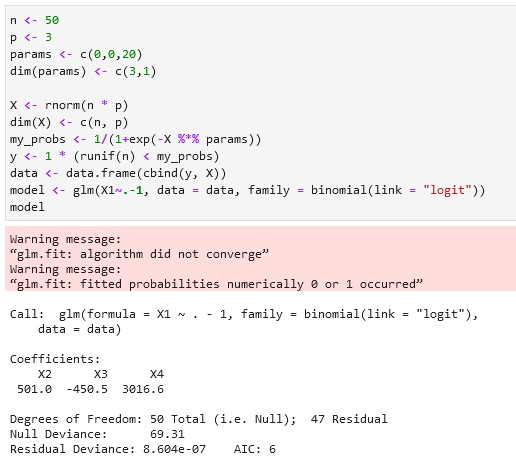
\includegraphics[width=0.7\textwidth]{1} 
        \end{center}
        \caption{R code for using ``\texttt{glm}'' to fit a logistic regression model with completely separated data.}   
    \label{figure1}
\end{figure}

\begin{figure}
        \begin{center}
            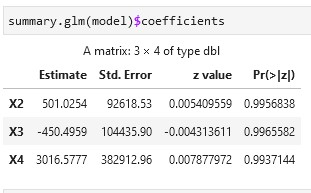
\includegraphics[width=0.5\textwidth]{2} 
        \end{center}
        \caption{R code for using ``\texttt{summary.glm}'' to obtain the $p$-value of the coefficients.}   
    \label{figure2}
\end{figure}


%We also conduct simulation studies which show that the proposed method outperforms the LRT in terms of both test level and test power.
%It is known that the LRT for these problems has nonstandard behavior.
%For these models, we prove that the generalized FBF has Wilks phenomenon.
%We also conduct simulation studies which show that the proposed method outperforms the LRT in terms of both test level and test power.

The reviwer noted that our original examples are too simple.
Indeed, the original normal mixture models have simple forms.
For these models, the proposed method is simple to compute and has regular behavior.
However, we would like to point out that the two normal mixture models and the binomial mixture model are irregular models and the LRT for these models are not very simple to use.
Take the second normal mixture model in the paper as an example.
For this model, the asymptotic distribution of the LRT is a difficult problem.
\cite{bickel1993} studied this problem, but they did not fully solve it.
\cite{LIU200461} gave the asymptotic null distribution of the LRT.
\cite{HALL2005158} derived the asymptotic power of the LRT.
According to the result of \cite{HALL2005158}, the LRT has trivial power under $n^{-1/2}$ local alternative hypothesis.
For this irregualar model, the generalized FBF still has Wilks phenomenon and has better performance than the LRT.
We think these examples can illustrate the advantages of the proposed method over the LRT.

It is interesing to use the proposed method to solve more complex and practical problems.
%But it is difficult to seriously investigate more problems within limited space.
We would like to leave it for future work.

\textbf{
    7. This paper is lack of tuning parameter selection which will be critical in the hypothesis testing result.
    Theoretically, it can satisfy some simple conditions, but in practice how to choose the tuning parameters $a$ and $b$ is very important.
}

\textbf{Answers:}
This question was raised by both reviewers.
Our Answer is as follow:

Our results imply that the choice of $a$ and $b$ does not affect the Wilks phenomenon and asymptotic power provided $a$ and $b$ are fixed and $0<b<a<1$.
In the simulation studies of the revised paper, the default value is $a=2/3$ and $b= 1/3$.
we also add a simulation to examine the effect of $a$ and $b$ on the finite sample performance of the test procedure.
It turns out that the proposed methdod is not sensitive to the choice $a$ and $b$.
In practice, if there is no practical evidence for the choice of $a$ and $b$, one can simply choose $a = 2/3$ and $b = 1/3$.


\section{List of major changes}
\begin{itemize}
    \item 
    We add an example of logistic regression model.
%We proved that the proposed method has Wilks phenomenon in this problem.
    \item 
    We add an example of binomial mixture model.
%It is known that the LRT for this model has complicated behavior.
%We proved that the proposed method has Wilks phenomenon in this problem.
    \item
        We add simulations studies for the logistic regression model, normal mixture model and the binomial mixture model.
    \item
        We add the asymptotic distribution of the intrinsic Bayes factor.
    \item
        The literature review is improved.
    \item
        We add many remarks to explain our results and assumptions.
    \item
        We simplify some of the theoretical proofs.
\end{itemize}




\bibliographystyle{apalike}
\bibliography{mybibfile}

\end{document}
